\section{Widget Sales}

\subsection*{(a)}
\begin{lstlisting}[language=Python]
for idx in shuffled_indices:
    s = int(log["s"][idx])
    a = int(log["a"][idx])
    r = log["r"][idx]
    s_next = int(log["s"][idx + 1])
    a_idx = np.where(A == a)[0][0]

    target = r + gamma * np.max(Q[s_next])
    Q[s, a_idx] += alpha * (target - Q[s, a_idx])
\end{lstlisting}
% Following the value-based RL update from lecture, I used tabular Q-learning on
% the historical data. For each recorded transition \((s_t,a_t,r_t,s_{t+1})\), the
% update was
% \[
% Q(s_t,a_t)\leftarrow Q(s_t,a_t)
% +\alpha\left(r_t+\gamma\max_{a'}Q(s_{t+1},a')-Q(s_t,a_t)\right)
% \]
% This is model-free because it only uses the sampled data and does not need the
% demand distribution.

\subsection*{(b)}
\begin{lstlisting}[language=Python]
Q_new = np.zeros_like(Q_vi)
for s in S:
    for a_idx, a in enumerate(A):
        expected_value = 0.0
        for d, p in zip(D, P):
            s_next = transition(s, a, d)
            expected_value += p * (reward(s, a, d) + gamma * np.max(Q_vi[s_next]))
        Q_new[s, a_idx] = expected_value
Q_vi = Q_new
\end{lstlisting}

% For value iteration, I used the model from the intern and applied the Bellman
% backup over the demand distribution:
% \[
% Q(s,a)\leftarrow
% \sum_d p(d)\left(r(s,a,d)+\gamma\max_{a'}Q(f(s,a,d),a')\right)
% \]
% Value iteration converged after 143 iterations.

\begin{figure}[H]
\centering
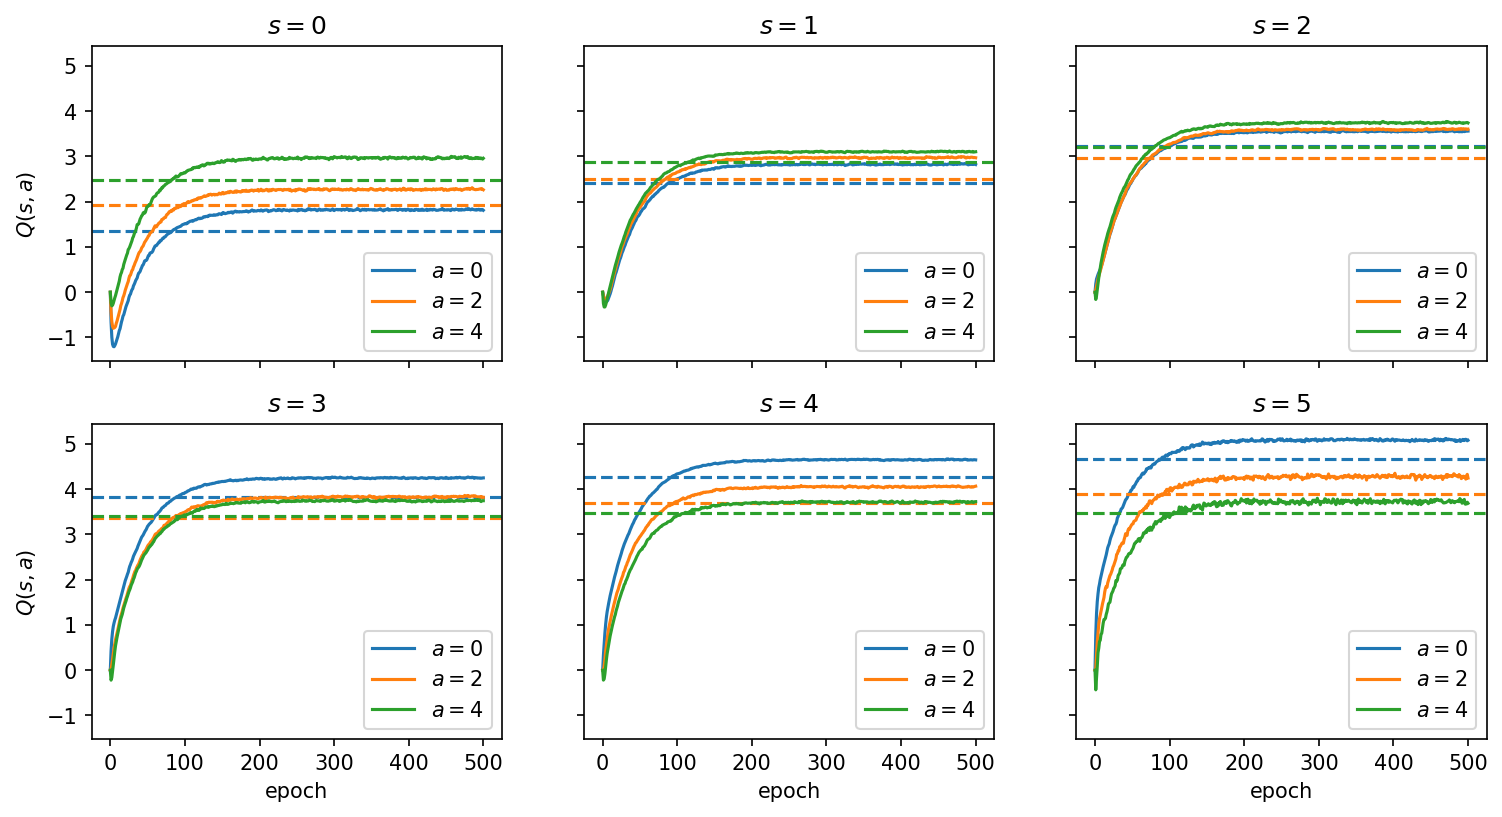
\includegraphics[width=\textwidth]{figures/widget_sales_qvalues.png}
\caption{Q-learning estimates vs value-iteration Q-values}
\label{fig:widget_qvalues}
\end{figure}

The Q-learning values approach the value-iteration values but do not match
exactly. This is expected because Q-learning only sees a finite logged dataset
generated by a random policy, while value iteration uses the exact demand model
and averages over all possible demands.

\subsection*{(c)}
\begin{lstlisting}[language=Python]
T = 5 * 365

a_opt_ql = A[np.argmax(Q, axis=1)]
a_opt_vi = A[np.argmax(Q_vi, axis=1)]

policy_ql = lambda s: a_opt_ql[int(s)]
policy_vi = lambda s: a_opt_vi[int(s)]

_, _, r_ql = simulate(np.random.default_rng(seed), policy_ql, T)
_, _, r_vi = simulate(np.random.default_rng(seed), policy_vi, T)

profit_ql = np.cumsum(r_ql)
profit_vi = np.cumsum(r_vi)
\end{lstlisting}

The optimal policies are:
\begin{lstlisting}[language=Python]
Optimal policy (Q-learning):      [4 4 4 0 0 0]
Optimal policy (value iteration): [4 4 0 0 0 0]
\end{lstlisting}

\begin{figure}[H]
\centering
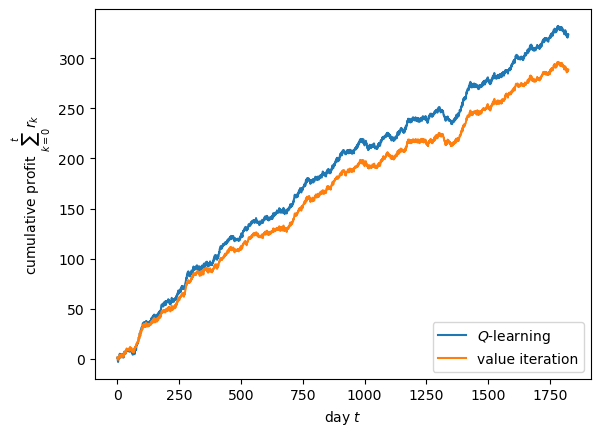
\includegraphics[width=0.75\textwidth]{figures/widget_sales_profits.png}
\caption{Cumulative profits over five years}
\label{fig:widget_profits}
\end{figure}

The Q-learning policy ended with cumulative profit
\(\sim 320\), while the value-iteration policy ended with cumulative profit
\(\sim 280\). The Q-learning policy orders more aggressively at \(s=2\), which
happens to do better on this sampled demand sequence. Value iteration is still
the cleaner policy in expectation because it is computed from the full demand
model, while the Q-learning policy is shaped by finite logged data.

